\section{Pianificazione}
Lo sviluppo del progetto è suddiviso nelle seguenti fasi:
    \begin{itemize}
        \item  RTB
        \item PB
    \end{itemize}
    \subsection{RTB}
    Nel periodo dal 04/11/2024 al 17/01/2025 verranno prodotti i seguenti documenti:
        \begin{itemize}
            \item "Norme di progetto"
            \item "Piano di progetto"
            \item "Analisi dei requisiti"
            \item "Piano di qualifica"
            \item "Glossario"
        \end{itemize}
    Inoltre verrà realizzato il Proof of Concept, per valutare la fattibilità tecnologica del progetto.
        \subsubsection{Sprint 1 (dal 11/11/2024 al 22/11/2024)}
        In questo periodo verrà definito il way of working, documentato nelle
        \textit{"Norme di progetto"}. Per quanto riguarda la gestione di progetto, verranno 
        pianificate le attività, stilato un preventivo e analizzati i rischi che potrebbero
        incidere sullo svolgimento del progetto. Infine si comincerà a redigere il 
        \textit{"Glossario"}, fondamentale per garantire una chiara comprensione e comunicazione all'
        interno del team e con il proponente.
        \\
        \begin{figure}[h!]
            \centering
            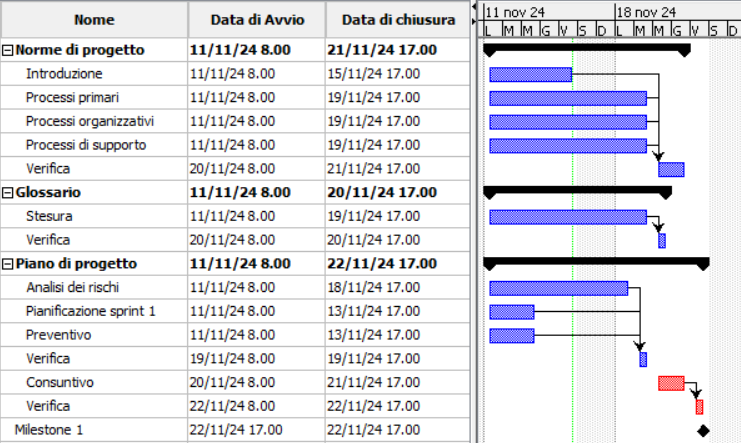
\includegraphics[scale = 0.85]{template/images/gantt1.png}
            \caption{Diagramma di Gantt sprint 1}
            \label{fig:3.1} % Etichetta per il riferimento
        \end{figure}

        \subsubsection{Sprint 2 (dal 25/11/2024 al 06/12/2024)}
        Durante questo secondo sprint, ci dedicheremo alla raccolta e all'analisi dei requisiti, identificando i 
        casi d'uso. Questi saranno documentati nel file \textit{"Analisi dei requisiti"} per garantire una visione 
        chiara degli obiettivi del progetto. Continueremo inoltre l'espansione del \textit{"Glossario"}, già 
        avviato durante lo sprint 1.  Procederemo con l'aggiornamento delle \textit{"Norme di Progetto"} tramite modifiche e miglioramenti per assicurare una gestione ottimale delle attività e delle risorse. Infine, con priorità minore, inizieremo la stesura del \textit{"Piano di Qualifica"}, necessario per definire le metriche e le modalità di 
        verifica della qualità del prodotto.

        
        \begin{figure}[h!]
            \centering
            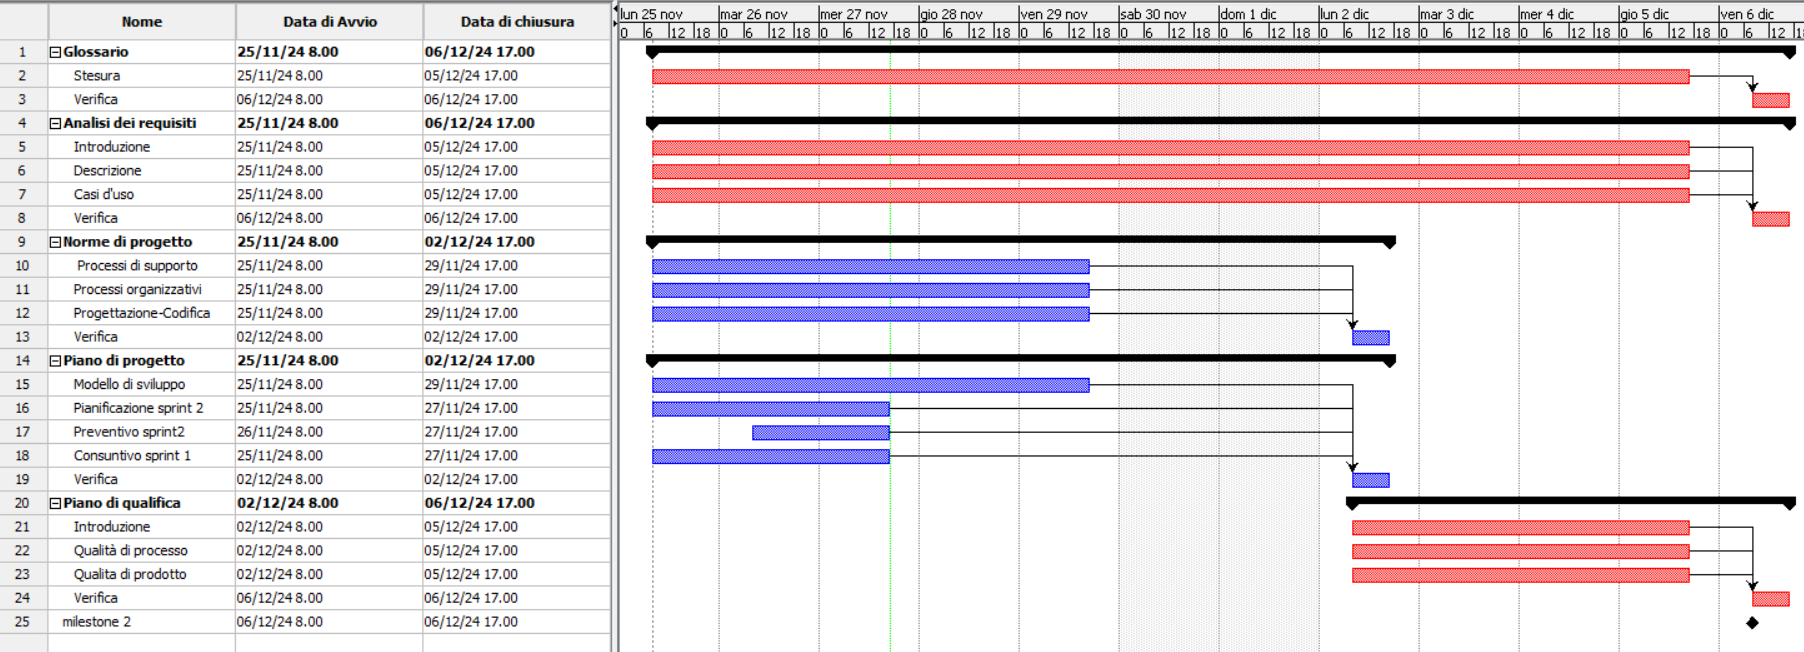
\includegraphics[scale = 0.3]{template/images/gantt2.png}
            \caption{Diagramma di Gantt sprint 2}
            \label{fig:3.2} % Etichetta per il riferimento
        \end{figure}


        \subsubsection{Sprint 3 (dal 9/12/2024 al 20/12/2024)}
        In questo terzo sprint continueremo l'aggiornamento delle \textit{"Norme di Progetto"} modificando e migliorando le regole che il team si pone di rispettare per garantire
        una gestione ottimale delle risorse e un metodo di sviluppo efficace ed efficiente. E' prevista inoltre la stesura delle metriche relative alla qualità del progetto e alla qualità del prodotto all'interno del documento \textit{"Piano di Qualifica"}.
        Successivamente, in quanto di minore importanza, è prevista la stesura delle metriche di testing sempre all'interno dello stesso documento.
        Per quanto riguarda il file\textit{"Analisi dei requisiti"} è pianificata la stesura dei requisiti funzionali e di qualità ed eventualmente, a seguito di un consulto con il proponente, si procederà anche con la stesura dei requisiti di vincolo e prestazionali.
        Infine è prevista l'espansione del \textit{"Glossario"}.

        \begin{figure}[h!]
            \centering
            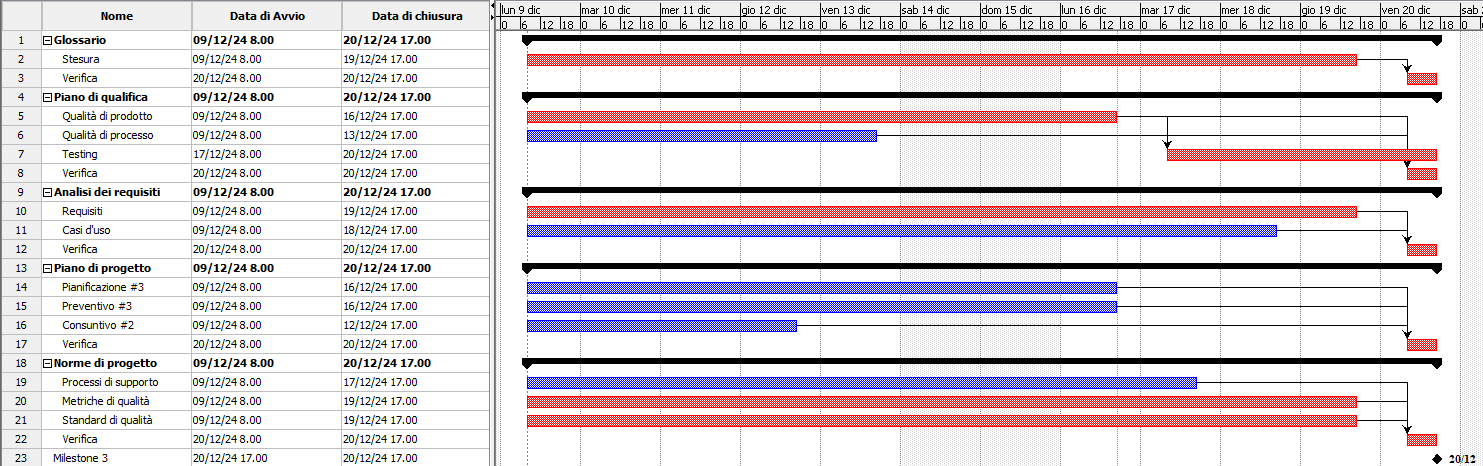
\includegraphics[scale = 0.3]{template/images/gantt3.png}
            \caption{Diagramma di Gantt sprint 3}
            \label{fig:3.3} % Etichetta per il riferimento
        \end{figure}

        \subsubsection{Sprint 4 (dal 23/12/2024 al 10/01/2025)}
        Durante questo quarto sprint (di durata maggiore a causa delle festività natalizie e della fine dell'anno), ci dedicheremo alla sistemazione dei casi d'uso, con l'obiettivo di garantire che siano coerenti, completi e allineati ai requisiti del progetto. 
        Una delle attività di maggiore importanza sarà la realizzazione del \textit{Proof of Concept} (PoC), che servirà a validare le scelte tecniche adottate e a dimostrare la fattibilità delle soluzioni individuate. 
        Parallelamente, si cercherà una soluzione per implementare in automatico il controllo della qualità della documentazione prodotta tramite Indice di Gulpease. 
        Infine, proseguiremo con l'espansione del Glossario, arricchendolo con nuovi termini e garantendo una migliore uniformità terminologica nel progetto.

        \begin{figure}[h!]
            \centering
            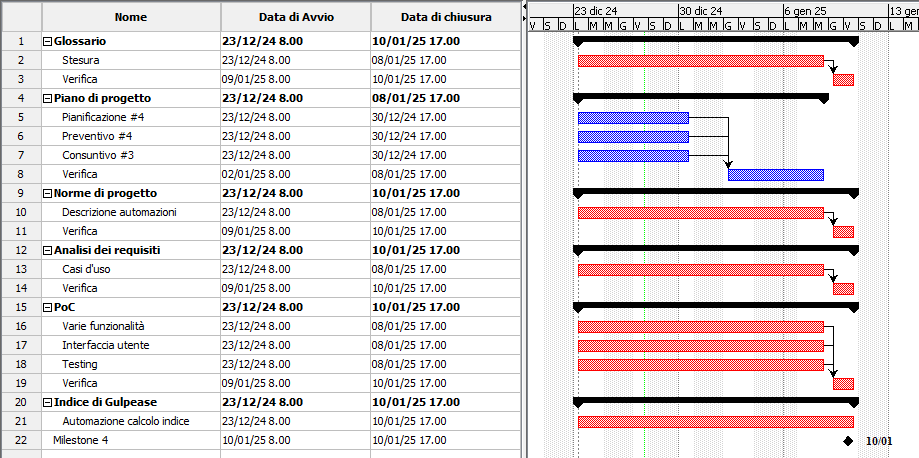
\includegraphics[scale = 0.45]{template/images/gantt4.png}
            \caption{Diagramma di Gantt sprint 4}
            \label{fig:3.4} % Etichetta per il riferimento
        \end{figure}

        \subsubsection{Sprint 5 (dal 13/01/2025 al 24/01/2025)}
        In questo sprint ci dedicheremo alla revisione e al completamento dei documenti necessari per la RTB.
        \\In particolare, andremo a migliorare la scrittura dei documenti che non hanno ottenuto un indice di Gulpease abbastanza alto, per fare in modo che la relativa metrica venga superata.
        \\Aggiungeremo le sezioni mancanti all'interno delle \textit{Norme di progetto} e rivedremo l'\textit{Analisi dei requisiti}, apportando modifiche ai casi d'uso e alla relativa rappresentazione tramite diagrammi UML.
        \\Ci occuperemo di arricchire ancor di più il \textit{Glossario}.
        \\Per quanto riguarda il \textit{Proof of Concept} (PoC), verranno dedicate alcune ore alla risoluzione degli ultimi bug grafici.

        \begin{figure}[h!]
            \centering
            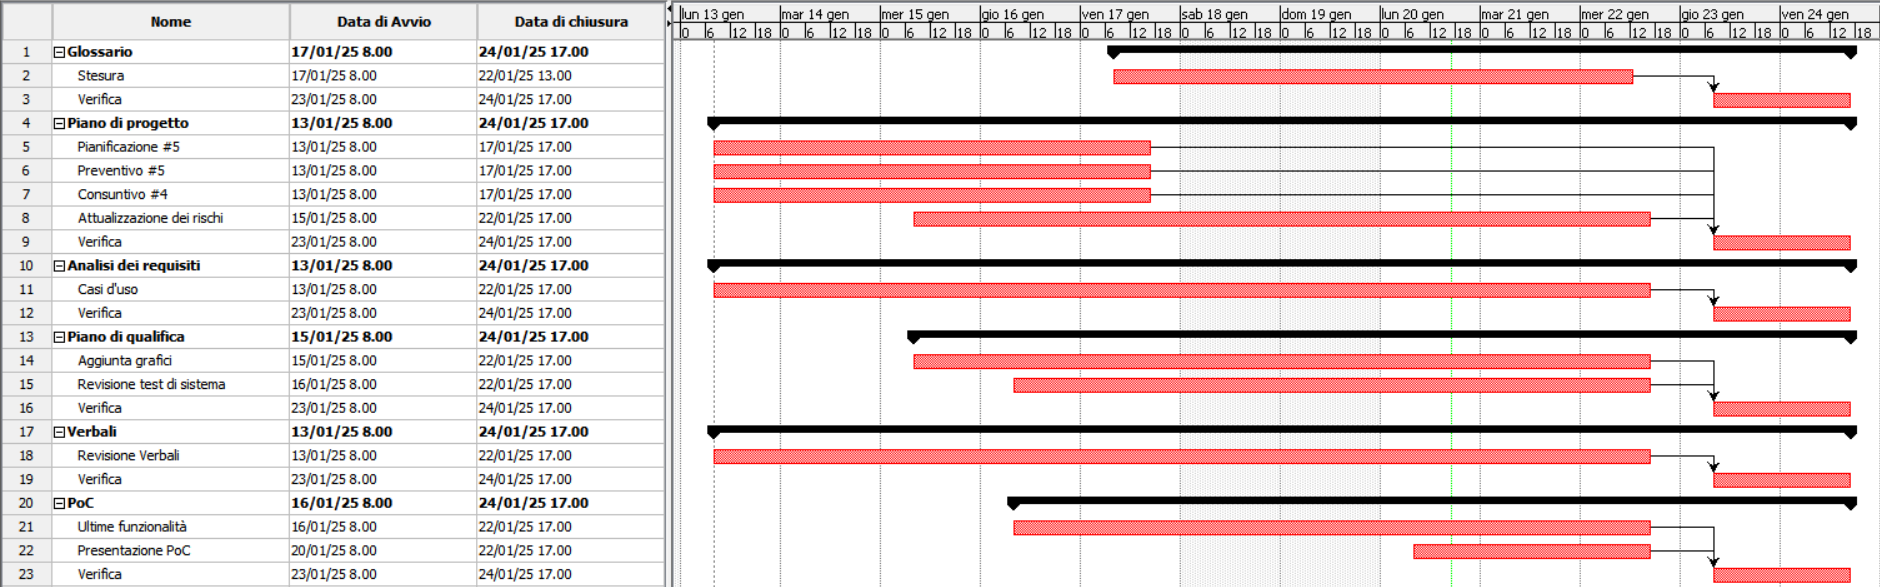
\includegraphics[scale = 0.4]{template/images/gantt5.png}
            \caption{Diagramma di Gantt sprint 5}
            \label{fig:3.4} % Etichetta per il riferimento
        \end{figure}

 
